\section{传播可辨识性：应优先研究的理论核心}
\subsection{当前观测与下游任务必须分别定义}
用 $F:\Theta\to\mathcal Y$ 表示\emph{实际}采集映射，用 $H:\Theta\to\mathcal Z$ 表示所需任务响应。$\Theta$ 包含合法材料和必要 nuisance。

无目标实验时，可定义 $F_{\rm cal}(W)=R G_WQ$；存在未知目标时则必须使用 $F_{\rm joint}(W,X,\gamma)$。早时窗数据也仍来自完整场，只是被时间窗算子处理。若窗外响应泄漏或深层最早到时未知，不能把窗口输出直接命名为“纯墙体散射”。

$H$ 可以是一个指定目标的完整响应、某任务域的传播签名，或最终目标位置泛函。区分这些选择是可辨识性结论成立的前提。

\subsection{纤维判据、局部条件与非线性障碍}
\begin{proposition}[观测纤维上的任务因子化，已知基本事实]
存在集合意义上的 $h:F(\Theta)\to\mathcal Z$ 使 $H=h\circ F$，当且仅当
\[
F(\theta_1)=F(\theta_2)\ \Longrightarrow\
H(\theta_1)=H(\theta_2).
\]
\end{proposition}
\begin{proof}
必要性直接。充分性是在每个观测纤维上选取一个代表，定义 $h(F(\theta))=H(\theta)$；纤维常值保证与代表无关。此论证不自动保证 $h$ 连续、可测或稳定。
\end{proof}
该命题是组织研究的问题定义，不是新的 Maxwell 定理。真正难点是特定材料类、采集配置下是否常值，以及噪声放大有多大。

若 $F,H,h$ 可微，令 $A=DF(\theta)$、$K=DH(\theta)$，则必须有
\[
\ker A\subseteq\ker K.
\]
有限维中，该条件等价于存在有限 $c$ 使
\[
\|Kv\|\le c\|Av\|\quad\forall v,\qquad
c_{\min}=\|KA^\dagger\|.
\]
证明是 $K=KA^\dagger A$，且 $A^\dagger$ 在 $\range A$ 上有界。$c$ 很大时，精确可辨识与实际稳定恢复仍然分离。

无限维中核包含不足以保证稳定性：在 $\ell^2$ 上取 $(Av)_j=v_j/j$、$K=I$，两者均无核，但 $K A^\dagger$ 无界。稳定性需要有界因子化，等价地需要
\[
K^*K\preceq c^2 A^*A
\]
等条件。网格有限维得到的常数可能随细化发散，不能称连续 Maxwell 的统一稳定证书。

\begin{example}[一阶条件不能替代非线性任务可辨识]
取 $F(x,z)=x$、$H(x,z)=z^2$。在 $(0,0)$ 有 $DH=0$，核包含成立；然而同一 $x$ 上任意小的 $z$ 变化都会改变任务。因此单点 Jacobian 检查不充分。
\end{example}

若 $F$ 在一个邻域恒秩，并且该邻域每一点均满足核包含，则在充分小的常秩坐标图中，$H$ 对纤维坐标的导数为零，因纤维切片连通而得到局部因子化。这才是将一阶条件积分为非线性结论的一种充分条件。动态弱奇异方向不自动构成可积分分布；若实际 Jacobian 满列秩，也不能强行画出正维 exact fiber。

\begin{proposition}[危险一阶方向的条件性非线性延拓]
在一个有限维材料参数化中，设 $\theta_0$ 为合法集合的内点，$F,H$ 为 $C^1$，$DF$ 在其邻域恒秩。若存在 $v\in\ker DF(\theta_0)$ 且 $DH(\theta_0)v\ne0$，则存在局部合法曲线 $\theta(t)$，使
\[
\theta(0)=\theta_0,\quad\theta'(0)=v,\quad
F(\theta(t))=F(\theta_0),\quad
H(\theta(t))=H(\theta_0)+tDH(\theta_0)v+o(t).
\]
\end{proposition}
\begin{proof}
常秩定理使局部水平集成为嵌入子流形，其切空间为 $\ker DF(\theta_0)$。在该子流形坐标图中取切向量 $v$ 对应的直线并映回；内点假设保证充分短的曲线保持合法。对 $H$ 作一阶展开即得结论。
\end{proof}
这是标准微分几何在当前问题上的条件性应用，不能声称已为任何具体 Maxwell 材料找到曲线。严格核与恒秩必须核实；微小但非零奇异值、被动性边界、硬拓扑变化或无限维网格极限均不由此覆盖。$F(t)=t^2$ 在零点的退化说明单点核并不足够。有限幅度、多拓扑和重要后验质量仍是独立问题。

\subsection{将目标与仪器补偿纳入可观测性}
实化白化后的联合线性化写为
\[
\delta y=J_W\delta w+J_X\delta x+J_\gamma\delta\gamma+e.
\]
令 $N=[J_X,J_\gamma]$。允许不受惩罚的局部补偿时，
\[
\min_{\delta x,\delta\gamma}
\|J_W\delta w+N(\delta x,\delta\gamma)\|^2
=\|(I-P_N)J_W\delta w\|^2.
\]
因此研究环境传播导数 $K_W=DH(W)$ 时，应比较
\[
A_{\rm vis}=(I-P_N)J_W,\qquad K_W.
\]
小的 $A_{\rm vis}v$ 与大的 $K_Wv$，才是“数据可被其他未知量补偿、但传播后果重要”的局部信号。只看原始 $J_W$ 会高估环境可辨识性。

若补偿有二次 prior 代价 $\Lambda_\nu\succ0$，有效数据加 prior 曲率为
\[
J_W^*\!\left[I-N(N^*N+\Lambda_\nu)^{-1}N^*\right]J_W.
\]
方括号一般不是正交投影。该 Schur 补描述局部 Gaussian/profile 近似，不能代替完整 nuisance 积分。有限变化仍须满足各频共享 nuisance、材料边界与 prior 范围。

可用于搜索的尺度化局部比率是
\[
\mathcal R(v)=
\frac{\|M_T^{1/2}K_Wv\|^2}
{\|A_{\rm vis}v\|^2+\lambda\|v\|_{M_{\rm prior}}^2}.
\]
$M_T$ 由任务损失定义，$M_{\rm prior}$ 由实际材料尺度或 prior 定义。它不是新 SVD 定理，也不是 posterior mass。不同参数单位必须通过 metric 同步变换，否则“大传播方向”可能只是坐标缩放。

\subsection{噪声尺度的非线性传播模数}
\begin{definition}[给定采集和材料类的任务歧义模数]
对声明的合法集合 $\Theta_0$，定义
\[
\omega_T(\delta;\Theta_0)=
\sup_{\substack{\theta_1,\theta_2\in\Theta_0\\
\|F(\theta_1)-F(\theta_2)\|_{\Sigma^{-1}}\le\delta}}
d_T(H(\theta_1),H(\theta_2)).
\]
\end{definition}
$\omega_T(0)=0$ 是精确任务可辨识；$\omega_T(\delta)\to0$ 是统一稳定任务可辨识。若 $\Theta_0$ 紧、$F,H$ 连续且纤维判据成立，可用紧性子列反证法证明该极限，但不保证良好的线性速率。

\textbf{科研价值在于为特定 Maxwell 条件提供非平凡界。} 找到一对合法世界即可给出 $\omega_T(\delta)$ 的下界。有限次搜索没找到，只能说当前搜索未给出见证；不能宣布 $\omega_T(\delta)=0$。如果 $\Theta_0$ 是“高后验质量集合”，其质量必须独立核验；不能把候选库自身定义成整个 posterior 支持。

\begin{proposition}[噪声下任务错误的二点下界]
将复数据实化，两个世界的分布为 $P_i=N(F_i,\Sigma)$，令
\[
d=\|F_1-F_0\|_{\Sigma^{-1}},\qquad
\Delta=d_T(H_1,H_0).
\]
对任意只使用当前数据的任务估计器，
\[
\max_{i=0,1}P_i\{d_T(\widehat H,H_i)\ge\Delta/2\}
\ge \Phi_{\rm N}(-d/2),
\]
其中 $\Phi_{\rm N}$ 是标准正态 CDF。
\end{proposition}
\begin{proof}
用估计结果较接近哪一个 $H_i$ 构造二元检验。若任务误差小于 $\Delta/2$，该检验必正确。共同协方差 Gaussian 两均值的等先验最优检验错误率为 $\Phi_{\rm N}(-d/2)$；最大错误概率不小于平均错误概率。
\end{proof}
于是平方风险至少有松下界 $(\Delta^2/4)\Phi_{\rm N}(-d/2)$。当 $d=0$ 且任务在 Hilbert 空间中，用平行四边形恒等式可加强到最大均方风险 $\Delta^2/4$。这些是标准统计工具。本文可能的物理贡献在于合法 Maxwell 世界产生的 $d,\Delta$，而不是重命名统计不等式。

\subsection{精确非磁 Maxwell 反例：相同反射、不同双程传播}
\paragraph{场景和观测。}
取真空两侧的无限平面、无损、非磁介质板，法向入射，频率 $\omega_0$。真空波长 $\lambda_0$，板折射率 $n>0$、厚度 $d$；两块板具有相同前表面 $z=0$。当前校准观测是该频率的复反射系数。此处首先是明确的无目标实验，不从实际联合观测中假造纯墙数据。

设 $\rho=(1-n)/(1+n)$、$\varphi=nk_0d$。全部内部反射求和给出
\[
r=\rho\,\frac{1-e^{2i\varphi}}{1-\rho^2e^{2i\varphi}},
\qquad
t_{0\to d}=\frac{(1-\rho^2)e^{i\varphi}}
{1-\rho^2e^{2i\varphi}}.
\]
当 $\varphi=\pi$，$r=0,t_{0\to d}=-1$。取
\[
W_1:\ (n_1,d_1)=(2,\lambda_0/4),\qquad
W_2:\ (n_2,d_2)=(3,\lambda_0/6).
\]
两者 $\epsilon_r$ 分别为 $4,9$，被动、非磁，且 $n_id_i=\lambda_0/2$，因此 $r(W_1)=r(W_2)=0$。

\paragraph{关键参考面。}
在相同的后方固定平面 $D>\max d_i$ 比较透射：
\[
t_D(W_i)=-e^{ik_0(D-d_i)},\qquad
\frac{t_D(W_2)}{t_D(W_1)}=e^{i\pi/6}.
\]
所以双程响应的比值为 $e^{i\pi/3}$，不会因往返而抵消。若误用两块同厚度板、只令透射差一个负号，平方后差异消失；那不是目标成像反例。

\paragraph{完整强目标。}
把反射系数为 $r_X$ 的平面目标放在 $z=L>D$。在一般频率，精确级联为
\[
y=r_L+
\frac{t^2 r_Xe^{2ik_0(L-d)}}{1-r_Rr_Xe^{2ik_0(L-d)}}.
\]
在上述共振频率，$r_L=r_R=0$，故
\[
y(W_i,L)=t_D(W_i)^2r_Xe^{2ik_0(L-D)}.
\]
因此
\[
|y(W_2,L)-y(W_1,L)|=|r_X|.
\]
允许 $r_X=-1$ 的 PEC 平面，完全不需要 Born 弱目标假设。墙内部的多次反射已精确包含。

\paragraph{联合位置补偿。}
再令 $L_2=L_1-\lambda_0/12$，则
\[
y(W_2,L_2)=y(W_1,L_1).
\]
这是两个墙材料和目标位置均不同、但单频单侧完整联合观测相同的世界。若先错误固定 $W_2$，目标位移可以吸收传播误差，而数据残差仍为零。

\paragraph{严格边界。}
该反例是完整 Maxwell 的一维子问题见证，不满足有限横向支撑的不规则墙体条件，且只在中心频率精确成立。它排除普遍的“先拟合墙回波就一定能正确成像”的主张；不能证明任意现实宽带阵列都具有同样歧义。定性现象也已有多模传输歧义先例。\cite{L_Waagaard}

\subsection{本轮实际运行的核验与一个重要负结果}
用独立传输矩阵实现检查上述公式，$\lambda_0=1$，固定 $D=1$，$L_1=1.5$，$L_2=1.5-1/12$，PEC 目标。结果如下：
\begin{itemize}
\item 中心频率最大墙反射模：$1.63\times10^{-16}$。
\item 同一目标位置的单位双程传播差模：$1.0000000000000004$。
\item 双程相位差：$1.0471975512=\pi/3$。
\item 目标位置补偿后联合响应差：$2.45\times10^{-16}$。
\item 三种板配置、1001 频率点的无损散射矩阵最大幺正性缺陷：$8.89\times10^{-16}$。
\end{itemize}
这些数值是代数实现核验，不是二维成像指标。

每个带宽配置使用 9 个等间距频率，实部/虚部各 $\sigma=0.01$ 的独立噪声；下表 $d$ 是\emph{两个无噪声均值之差}的白化距离，不是拟合残差与 $\sqrt{\dim y}$ 的比较。
\begin{center}
\begin{tabular}{rrrrr}
\toprule
相对全带宽 & 墙校准 $d$ & 校准最优错误率 & 联合补偿对 $d$ & 双程差 RMS\\
\midrule
$0.2\%$ & $0.355$ & $0.430$ & $1.217$ & $1.000$\\
$0.5\%$ & $0.887$ & $0.329$ & $3.038$ & $1.000$\\
$1\%$ & $1.774$ & $0.188$ & $6.055$ & $1.000$\\
$2\%$ & $3.545$ & $0.038$ & $11.942$ & $1.000$\\
$5\%$ & $8.809$ & $5.30\!\times10^{-6}$ & $27.215$ & $0.998$\\
\bottomrule
\end{tabular}
\end{center}

\textbf{关键负结果：} $0.5\%$ 带宽下，这一对墙的校准数据仍难分，但既定的墙加 PEC 位移补偿对已经有 $d=3.038$；到 $1\%$ 时 $d=6.055$。完整联合数据会击破这组特定补偿。不能用校准 $d=0.887$ 代替联合问题的可辨识性。这正说明 P0 必须同时跑 calibration 与 joint 两种定义。

固定 9 点随带宽重新布点不是嵌套采集；因此某个距离随带宽局部下降不违反新增独立观测的信息单调性。全带宽为零的一行可解释为同频独立重复，仍没有区分该 exact pair 的信息。

\begin{figure}[ht]
\centering
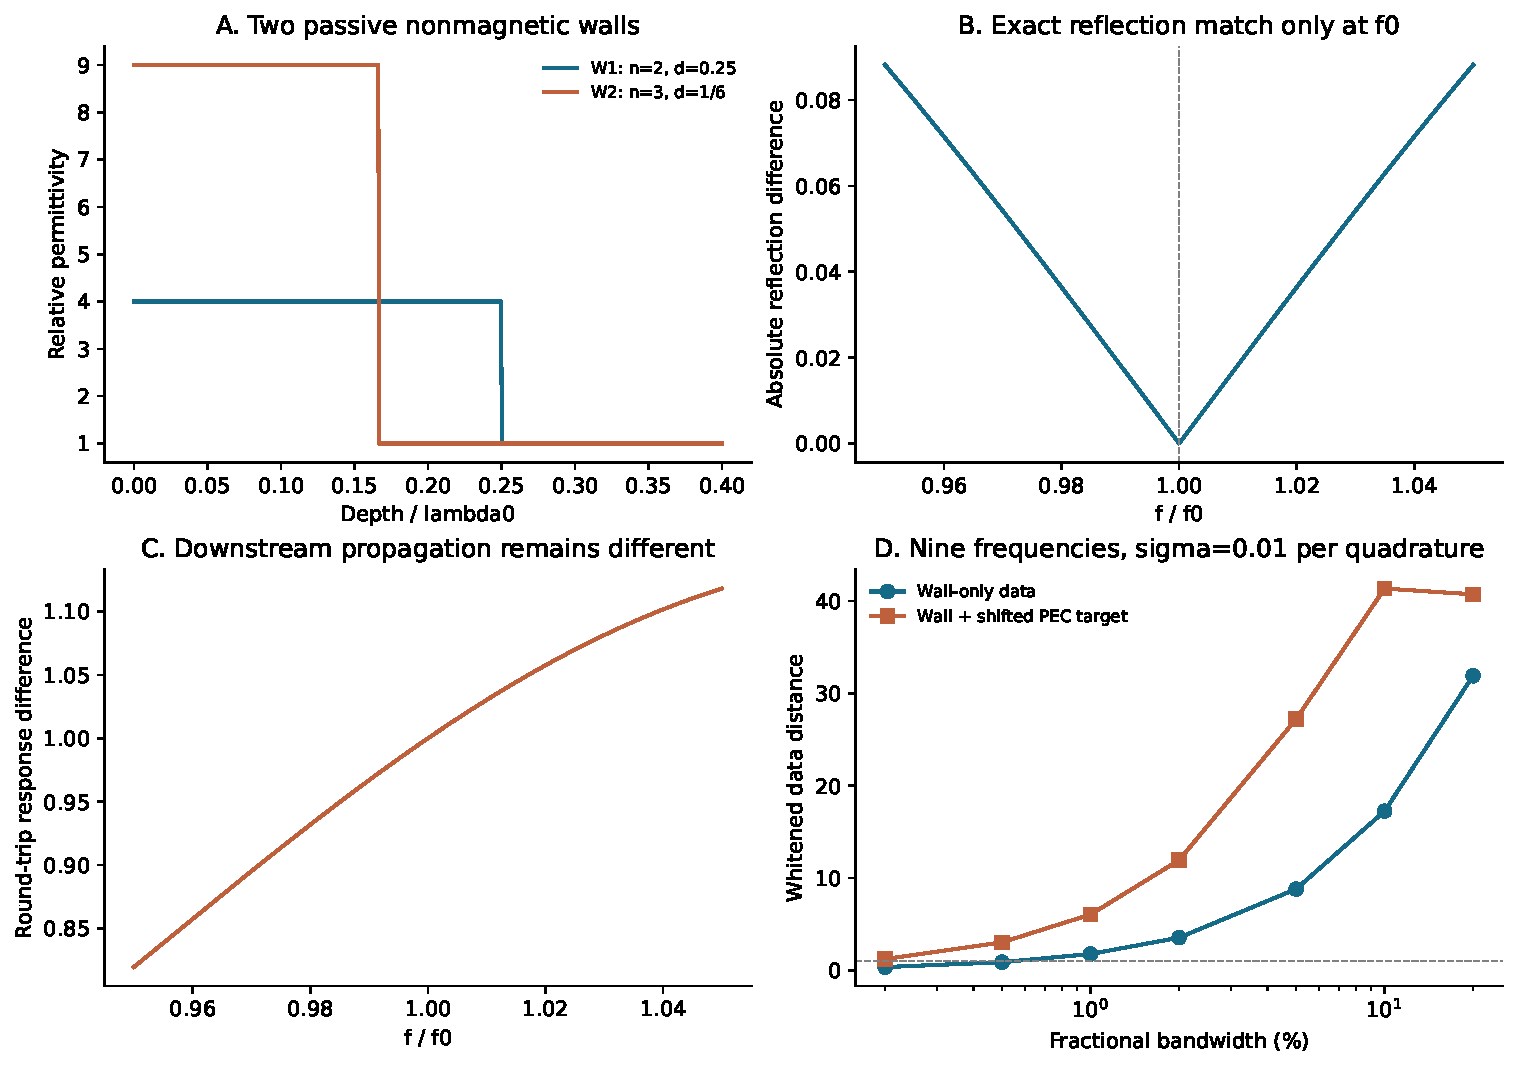
\includegraphics[width=.98\linewidth]{../analytic_results/exact_maxwell_witness.pdf}
\caption{本轮已执行的一维精确 Maxwell 核验。不同厚度的共振板在中心频率反射相同；同参考面双程传播不同。有限带宽破坏该特定联合补偿，不把此图当作二维复杂墙体结果。}
\end{figure}

\subsection{补偿、可辨识充分条件和真正的失败边界}
墙厚与折射率的光程、界面反射幅度、目标位置、复散射强度和仪器相位可相互影响。只有光程近似相同并不足以保证全波数据相同；空腔与等效低介电区也只在特定长波极限近似等效，界面散射、色散与多次反射会打破等效。金属增强结构的路径变化同理，必须计算完整响应。

一种充分条件是总材料 $m$ 在声明数据类中唯一且稳定可恢复，并且 $H(m)$ 在该类上 Lipschitz；则复合映射给任务稳定性。更弱条件只要求任务在纤维上常值。连续边界 Maxwell 数据的部分数据唯一性文献说明，不能笼统说“单侧必然不可辨”；其允许的激励、几何与完整边界响应，远强于有限天线采样。\cite{L_Partial,L_Zhai}

有限孔径在 Born 极限中限制被采样空间频率；全非线性多次散射可能带入附加耦合，也可能恶化 conditioning。因此 Born 缺角结论是机制解释，不能直接充当全非线性严格核空间结论。

另一个独立失败机制是屏蔽：闭合理想 PEC 屏障内的外部不可达目标不能由外部照明恢复；这时相应可测目标响应本身为零。高损耗或高反射层使双程幅度极小，任务 Fisher 信息相应衰减。它与“墙回波相似但透射行为不同”是两种机制，不应混称。

\subsection{错误墙模型如何传递到定位}
在真实世界附近，若强行固定 $\widehat W=W_*+\delta w$，且目标数据映射足够光滑，局部最小二乘给
\[
\delta x\approx J_X^\dagger(n-J_W\delta w).
\]
若相关目标可观测子空间最小奇异值 $s_X>0$，则局部
\[
\|\delta x\|\lesssim
s_X^{-1}\left(\|n\|+\|J_W\delta w\|\right)
+\text{受控二阶项}.
\]
有 nuisance 时须先消去其可补偿分量。带正则时应写 $(J_X^*J_X+\Lambda_X)^{-1}J_X^*$，同时承认 prior 偏差。多个目标模式、目标出现/消失、相位周期歧义或 $s_X\to0$ 时，这个局部界失效。不能只给传播误差一个小数字，就宣称定位误差也小。

